\chapter{Applying the coupling}\label{ch:c7}
This chapter takes the user from data to a calibrated coupled model: a complete worked example with the Liard River model,
how to prepare data for another basin, a checklist and typical parameter values, calibration, and troubleshooting.

\begin{plain}
This chapter walks through a real example --- the Liard River in northern Canada --- from input files to results. It then
shows how to set up your own watershed, which values to start from, how to calibrate, and what to do when something goes
wrong.
\end{plain}

\section{Tutorial: the Liard River model}\label{ch:tutorial}
This chapter walks through the example supplied in \cmd{examples/Liard\_groundwater}: the Liard River model (65 subbasins,
1\,107 HRUs, northern British Columbia and Yukon) with an aquifer added under three nested subbasins (52, 48 and 43;
about 13\,800 km$^2$, 85 coupled HRUs). The other 62 subbasins run exactly as they do without groundwater.

\subsection{Step 0: prepare}
\begin{enumerate}
\item Get Raven with the coupling (RavenHydroFramework; until the pull request is merged, the \cmd{mf6-coupling} branch
of \url{https://github.com/rarabzad/RavenHydroFramework}) and, beside it, RavenHydroFramework-extra (branch \cmd{main} of
\url{https://github.com/rarabzad/RavenHydroFramework-extra}; Section~\ref{sec:building}). Build Raven with CMake: \cmd{cmake -S . -B build}, \cmd{cmake --build build
--config Release} (an optimised \cmd{Release} build by default). With a Fortran compiler, meson~$\geq$~1.7, ninja and git,
and the MODFLOW~6 repository reachable, this also builds the MODFLOW~6 library from source; otherwise (also offline) it
downloads the official release library (Linux x86\_64, Windows x64, Apple Silicon Macs); either
way the library ends up next to Raven, which finds it without any setting (Section~\ref{sec:building}).
\item If Raven was built without the library (\cmd{make} in \cmd{src/}, \cmd{src/Raven.sln}, \cmd{-DRAVEN\_MF6=OFF}, or
the configure warned that it found no way to get it), get it (6.5 or newer; tested with 6.8.1 and 6.6.3; 6.8 or newer
recommended) with \cmd{python tools/get\_mf6.py} in the RavenHydroFramework-extra repository
(Section~\ref{sec:getmf6}). \cmd{get\_mf6.py} has no library for Linux other than x86\_64 (e.g.\ aarch64), for Windows on
ARM64, or for Intel Macs (only with \cmd{--version 6.6.3}); there, build it with Raven: \cmd{cmake -S . -B build
-DRAVEN\_MF6=SOURCE}, or give a library you have with \cmd{-DRAVEN\_MF6=PATH -DRAVEN\_MF6\_PATH=/path/to/libmf6.so}.
\item The original Liard package was made for Raven 2.9.1; for Raven 4.x its Windows paths use \texttt{/} and the parameter
\cmd{DEP\_THRESHHOLD} is spelled \cmd{DEP\_THRESHOLD}. The example files already include these changes.
\end{enumerate}

\subsection{Step 1: mark the HRUs with groundwater (.rvh)}
In the \cmd{:HRUs} table, the \cmd{AQUIFER\_PROFILE} column was filled for the HRUs of subbasins 52, 48 and 43:
\cmd{VALLEY\_ALLUVIUM} for forest, shrub and wetland HRUs; \cmd{UPLAND\_TILL} for barren HRUs; glaciers keep \cmd{[NONE]}.
A group listing the same HRUs was added at the end of the file:
\par\noindent\begin{minipage}{\linewidth}
\begin{lstlisting}
:HRUGroup AquiferHRUs
  2736, 2745, 2747, ...
:EndHRUGroup
\end{lstlisting}
\end{minipage}\par\smallskip

\subsection{Step 2: describe the aquifer (.rvp)}
Added at the end of \cmd{Liard.rvp}:
\begin{lstlisting}
:AquiferClasses
  :Attributes, K_HORIZ, K_VERT, SPEC_STORAGE, SPEC_YIELD, POROSITY
  :Units,      m/d,     m/d,    1/m,          none,       none
  GRAVEL,      50.0,    5.0,    1.0E-5,       0.25,       0.30
  CLAY_TILL,   0.001,   0.0001, 1.0E-4,       0.03,       0.40
  SAND,        10.0,    1.0,    1.0E-5,       0.20,       0.35
  UPLAND_TILL, 0.2,     0.02,   1.0E-4,       0.08,       0.30
:EndAquiferClasses

:AquiferProfiles
  VALLEY_ALLUVIUM, 3, GRAVEL, 15.0, AQUIFER, CLAY_TILL, 5.0, AQUITARD, SAND, TO_BEDROCK, CONFINED_AQUIFER
  UPLAND_TILL,     1, UPLAND_TILL, TO_BEDROCK, AQUIFER
:EndAquiferProfiles

:AquiferProfileParameters
  :Attributes,     INITIAL_HEAD_DEPTH, DEFAULT_BEDROCK_DEPTH, SEEPAGE_LEAKANCE, SOIL_ZONE_DEPTH
  :Units,          m,                  m,                     1/d,              m
  VALLEY_ALLUVIUM, 3.0,                60.0,                  1.0,              0.0
  UPLAND_TILL,     8.0,                15.0,                  1.0,              0.0
:EndAquiferProfileParameters
\end{lstlisting}
The valley aquifer is a gravel layer (15 m) over a clay-till aquitard (5 m) over sand down to bedrock; the uplands have one
till layer to shallow bedrock.

\subsection{Step 3: switch the coupling on and send recharge to it (.rvi)}
\par\noindent\begin{minipage}{\linewidth}
\begin{lstlisting}
:GroundwaterModel MODFLOW6
:DefineHRUGroups AquiferHRUs
...
:Percolation PERC_CONSTANT FAST_RESERVOIR SLOW_RESERVOIR
  :-->Conditional HRU_GROUP IS_NOT AquiferHRUs     # existing process, only for uncoupled HRUs
:Percolation PERC_CONSTANT FAST_RESERVOIR GROUNDWATER
  :-->Conditional HRU_GROUP IS AquiferHRUs         # new: this water becomes recharge
\end{lstlisting}
\end{minipage}\par\smallskip
Seepage returns to the lowest soil layer (\cmd{SLOW\_RESERVOIR}), whose existing baseflow process carries it to the rivers;
aquifer--river exchange goes directly to the reaches.

\subsection{Step 4: the groundwater file (.rvg)}
\begin{lstlisting}
#########################################################################
# Liard.rvg - Raven-MODFLOW 6 groundwater file (Liard River test case)
#   Groundwater under Central Liard subbasins 52 -> 48 -> 43 (85 HRUs).
#   Hydrogeology (aquifer classes, profiles) is in Liard.rvp;
#   which HRUs have groundwater is set by AQUIFER_PROFILE in Liard.rvh.
#########################################################################

# --- geometry (stand-in data built by tools_build_standin_inputs.py; replace with real data) ---
:HRUGeometry        Liard_HRUs_standin.geojson  HRU_ID    # HRU polygons, lon/lat
:RiverGeometry      Liard_rivers.geojson                  # river lines (subbasin assigned automatically)
:LandSurface        Liard_dem_standin.asc                 # DEM, ESRI ASCII, lon/lat
:BedrockSurface     Liard_bedrock_standin.asc             # bedrock elevation, same format

# --- grid and coupling settings ---
:GridCellSize       2000.0     # m
:MinCellCoverage    0.25       # fraction of a cell covered by coupled HRUs to activate it
:HeadSaveFrequency  365        # steps between saves of the full head field (mf6/gwf.hds)
# :MF6Library       /path/to/libmf6.so    # only if Raven does not find it by itself (or RAVEN_MF6_LIB)

# --- optional features (uncomment to use; see the user guide) ---
# :GWInitialization  STEADY_STATE 0.45            # steady-state start, uniform recharge [mm/d]
# :SurfaceWaterExchange DEPRESSION WetlandHRUs LEAKANCE 0.01   # wetlands <-> aquifer
# :WriteNetCDFHeads                               # GWHeads.nc (Raven built with -Dnetcdf)
# :ReservoirExchange                              # Raven reservoirs (with :SeepageParameters) <-> aquifer
# :Wells
#   :Attributes, NAME, LATITUDE, LONGITUDE, SCREEN_TOP, SCREEN_BOT
#   1, PW_1, 59.27310, -124.73460, 1199.7, 1188.7
# :EndWells                                        # rates: :WellFlowRate 1 m3/d ... in Liard.rvt
# :ObservationWells
#   :Attributes, NAME, LATITUDE, LONGITUDE, SCREEN_ELEV
#   101, OW_NEAR, 59.27310, -124.73060, 1192.7
# :EndObservationWells                             # data: :ObservationData GW_HEAD 101 m ... in Liard.rvt
# head boundaries: a HEAD (or a :BoundaryHead series in Liard.rvt) must lie above the bottoms of the cells it is to hold;
# the top layer under these two lies between about 1300 and 1315 m (3 GHB and 9 CHD cells with these heads)
# :GeneralHeadBoundary   GHB1 boundary_line.geojson HEAD 1310.0 CONDUCTANCE 5000.0 LAYERS TOP
# :SpecifiedHeadBoundary LAKE1 lake.geojson HEAD 1312.0 LAYERS TOP
\end{lstlisting}
The HRU polygons, DEM and bedrock of this example are \emph{stand-ins}: the Liard package has no HRU polygons, DEM or
bedrock map, so \cmd{tools\_build\_standin\_inputs.py} made Voronoi polygons around the HRU centroids clipped to each
subbasin, a DEM interpolated from HRU elevations, and bedrock 60 m (valley), 15 m (upland) and 5 m (glacier) below it.
For a real study, replace them with real data.

\subsection{Step 5: run}
\par\noindent\begin{minipage}{\linewidth}
\begin{lstlisting}
cd examples/Liard_groundwater
../../Raven.exe Liard -o output/
python3 tools_audit.py output        # optional automated check
\end{lstlisting}
\end{minipage}\par\smallskip
The 20-year daily run takes about 10 minutes on one processor core (35 seconds without groundwater). Raven builds a grid of
3 layers $\times$ 85 $\times$ 54 cells of 2 km, 3\,252 active columns, 178 river cells (Figure~\ref{fig:grid}).

\subsection{Step 6: look at the results}
\begin{itemize}
\item \cmd{GWModelSummary.txt}: check the grid, the number of active cells and that every coupled HRU is linked.
\item \cmd{GWBudget.csv}: the daily groundwater balance (Figure~\ref{fig:budget}); the error column should stay tiny.
\item \cmd{GWHRUState.csv}: depth to water under each HRU (Figure~\ref{fig:wtdepth} shows the map from \cmd{mf6/gwf.hds}).
\item \cmd{Hydrographs.csv}: streamflow includes groundwater discharge (Figure~\ref{fig:hydro}).
\end{itemize}
\begin{figure}[!htbp]\centering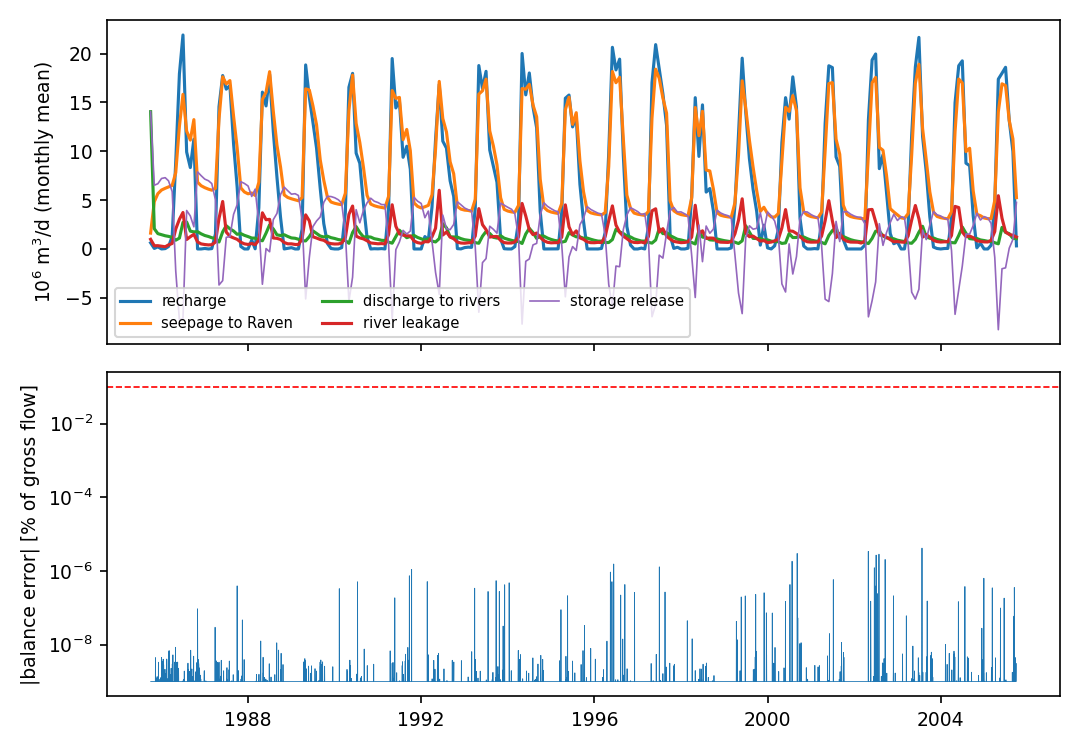
\includegraphics[width=\linewidth]{figures/fig_budget.png}
\caption{Groundwater budget of the 20-year Liard run (monthly means) and daily balance error; the dashed line is 0.1\%.}\label{fig:budget}\end{figure}
\begin{figure}[!htbp]\centering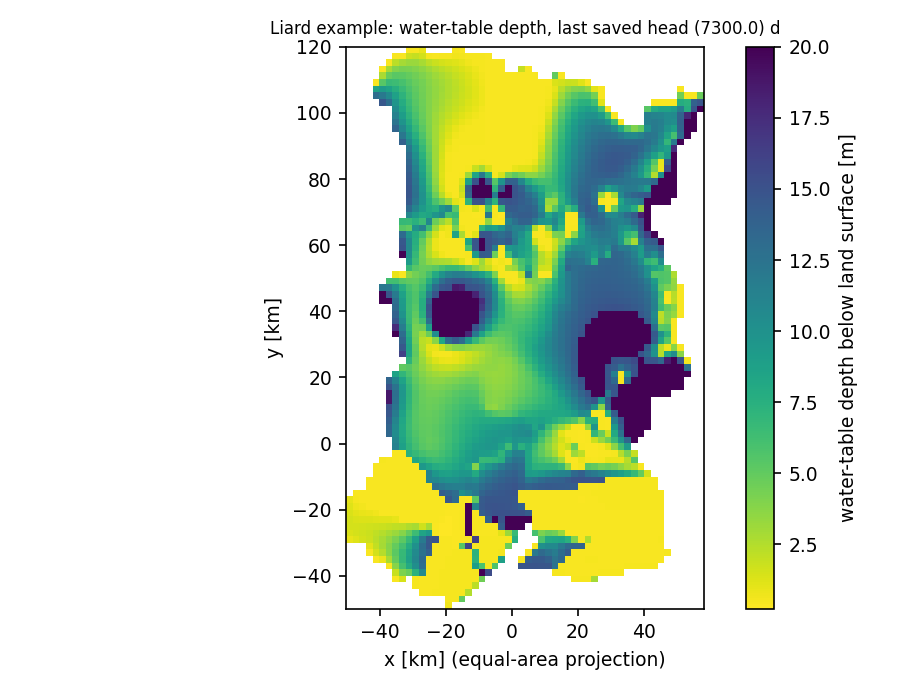
\includegraphics[width=0.72\linewidth]{figures/fig_wtdepth.png}
\caption{Depth to water at the last saved head.}\label{fig:wtdepth}\end{figure}
\begin{figure}[!htbp]\centering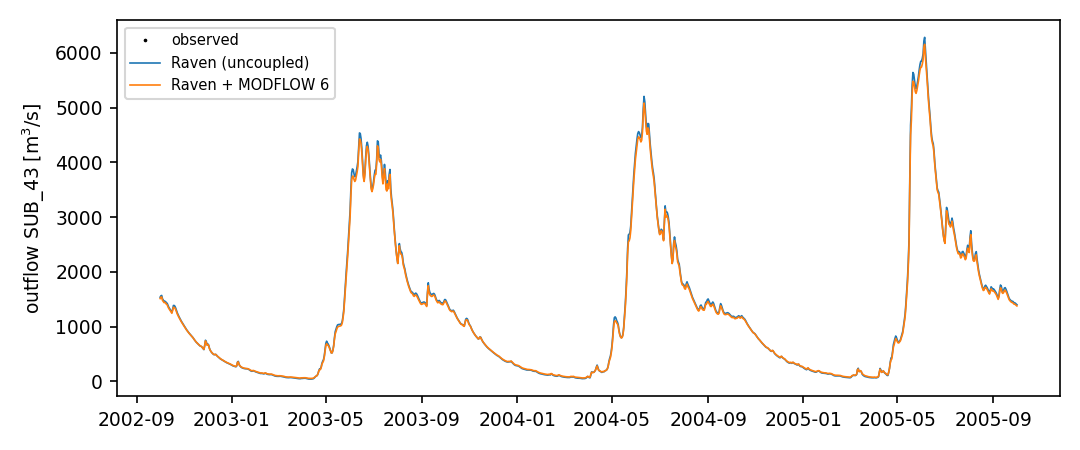
\includegraphics[width=\linewidth]{figures/fig_hydrograph.png}
\caption{Outflow of subbasin 43, 2003--2005, without and with groundwater (not recalibrated).}\label{fig:hydro}\end{figure}
Without recalibration and with stand-in geometry, the Nash--Sutcliffe efficiency at gauges 10BE004, 10BE005 and 10BE010
changes from 0.867, 0.835, 0.681 to 0.850, 0.821, 0.634. Recalibrating with flow and head data is the natural next step.

\section{Preparing the input data}
\subsection{HRU polygons}
Raven's HRUs usually come from a GIS overlay (for example BasinMaker): subbasins intersected with land-use, soil and terrain
classes. Export that polygon layer, keeping the HRU ID used in the \cmd{.rvh}:
\par\noindent\begin{minipage}{\linewidth}
\begin{lstlisting}
ogr2ogr -f GeoJSON -t_srs EPSG:4326 my_hrus.geojson my_hrus.shp
\end{lstlisting}
\end{minipage}\par\smallskip
(or, in QGIS, \emph{Export $\rightarrow$ Save Features As}, format GeoJSON, CRS EPSG:4326). A layer in a projection may also be
exported as it is (\cmd{ogr2ogr -f GeoJSON my\_hrus.geojson my\_hrus.shp}) and its projection given by \cmd{:InputCRS} in the
\cmd{.rvg} file (Section~\ref{sec:inputcrs}). Check that every HRU with an
\cmd{AQUIFER\_PROFILE} appears in the file; \cmd{GWModelSummary.txt} lists, per HRU, its polygon area, its area in the \cmd{.rvh}
and the fraction linked to active cells.
\subsection{Maps}
The DEM and the bedrock (or aquifer base) surface are GeoTIFF files or ESRI ASCII grids in longitude/latitude, for
example:
\par\noindent\begin{minipage}{\linewidth}
\begin{lstlisting}
gdalwarp -t_srs EPSG:4326 -tr 0.005 0.005 -r bilinear -dstnodata -9999 -co COMPRESS=DEFLATE dem.tif dem_lonlat.tif
\end{lstlisting}
\end{minipage}\par\smallskip
(\cmd{-dstnodata} marks the area outside the source as no-data, so that it does not read as 0~m.) Use a raster resolution finer than the model cells (each model cell averages 25 samples). A projected raster can be used
without warping, with \cmd{:InputCRS} giving its projection (Section~\ref{sec:inputcrs}); all input files then use that
projection, and the EPSG code of a GeoTIFF is checked against it. GeoTIFF files must hold one band and be uncompressed or
compressed with LZW, DEFLATE or PackBits (Section~\ref{sec:geotiff}); \cmd{gdal\_translate -b 1 -co COMPRESS=DEFLATE}
converts others. Both maps must use the same vertical datum, as must
well screens, monitoring wells, boundary heads and reservoir stages; the only automatic check is the start-up stop for a
coupled reservoir whose stages lie below the aquifer under its lake.
\subsection{River lines}
Any line layer of the river network in longitude/latitude (or in the projection of \cmd{:InputCRS}). A field with the Raven subbasin ID is optional; without it, each
river piece is assigned to the subbasin of the HRU that dominates its grid cell.
\subsection{Aquifer information}
Layer thicknesses and materials come from borehole logs, geological maps or regional hydrogeological studies. Start with one or
two profiles and typical values (Section~\ref{ch:ownmodel}); refine only where data or calibration demand it.

\section{Choosing a grid for the Liard model}\label{sec:liardgrids}
The Liard model was run for two years on each grid option (Table~\ref{tab:liardgrids}); every run keeps the water accounts
exact (MODFLOW residual about $10^{-11}$, no failed step, Raven's balance unchanged).
\begin{table}[!htbp]\centering
\caption{The Liard model (2 years) on each grid: active cells, run time on one core, Nash--Sutcliffe efficiency at 10BE004 /
10BE005 / 10BE010, mean seepage to Raven and mean net aquifer discharge to rivers [million m$^3$/d].}\label{tab:liardgrids}
\begin{tabular}{lrrcrr}\toprule\hdr
Grid & Cells & Time [s] & NSE & Seepage & Rivers\\\midrule
Regular 2 km (default) & 8\,840 & 40 & 0.728 / 0.861 / 0.635 & 9.48 & 0.82\\
Regular, rotated 20\textdegree, 1 km along rivers & 35\,058 & 220 & 0.726 / 0.861 / 0.638 & 9.92 & 0.66\\
Quadtree 2 km, 500 m along rivers & 16\,276 & 108 & 0.719 / 0.858 / 0.611 & 9.49 & 0.01\\
HRU mesh 2 km, 1 km along rivers & 14\,610 & 100 & 0.717 / 0.859 / 0.627 & 9.94 & 0.35\\
Regular 2 km, layers by elevation & 8\,840 & 41 & 0.666 / 0.859 / 0.606 & 4.11 & 0.49\\
\bottomrule\end{tabular}
\par\smallskip\footnotesize MODFLOW 6.8.1 (\cmd{tests/liard\_grids.py}); run times on one core of the test machine.
\end{table}
Streamflow hardly changes: total seepage is nearly the same on every grid and the river exchange is a small part of the
flow at the gauges. The net river exchange, however, depends on the size of the river cells --- 0.82 million m$^3$/d with
2 km cells, 0.01 with 500 m cells --- for two reasons: the channel bed is placed at the lowest DEM value along the river in
each cell, which is lower in larger cells, and the head of a large cell averages the aquifer over a wider area around the
river. Calibrate the riverbed parameters (\cmd{RIVERBED\_K}, \cmd{:RiverBedDepth}) on the grid that will be used, and
compare models only at the same river-cell size. Connecting layers by elevation halves the seepage here, because water in
the upland till can flow directly into the valley gravel where the two lie at the same elevation --- a different
conceptual model rather than a refinement. A regular grid refined to 1 km along rivers has more than twice the cells of a
quadtree with 500 m river cells, because its refinement spans whole rows and columns.

\section{Setting up your own model}\label{ch:ownmodel}
\subsection{Checklist}
\begin{enumerate}
\item \textbf{HRU polygons.} Export the HRU polygons from your GIS or BasinMaker as GeoJSON in longitude/latitude
(EPSG:4326), or in their projection with \cmd{:InputCRS}, with a field holding the HRU ID used in the \cmd{.rvh} file.
\item \textbf{Maps.} A DEM and a bedrock (or aquifer-base) elevation map as GeoTIFF files or ESRI ASCII grids in
longitude/latitude (or in the projection of \cmd{:InputCRS}), in the same vertical datum. River lines as GeoJSON.
\item \textbf{Profiles.} Group your HRUs by the aquifer beneath them and write one profile per group; set
\cmd{AQUIFER\_PROFILE} in the \cmd{.rvh}.
\item \textbf{Recharge.} Decide which Raven flux is recharge (usually percolation from the deepest soil store) and send it
to \cmd{GROUNDWATER} for coupled HRUs only. Remove or restrict any process that drains \cmd{GROUNDWATER} there, and any
conceptual baseflow that would double-count groundwater.
\item \textbf{Grid size.} Choose $\Delta$ so that the smallest features you care about span a few cells, but the number of
active cells stays manageable (a few thousand to a few hundred thousand per layer).
\item \textbf{Start.} Use \cmd{:GWInitialization STEADY\_STATE} with the long-term average recharge, or a warm-up period.
\item \textbf{Check.} Read \cmd{GWModelSummary.txt} and run \cmd{tools\_audit.py}.
\item \textbf{Calibrate.} Use streamflow and monitoring-well heads (Section~\ref{ch:calib}).
\end{enumerate}

\section{A water table in the soil, on sloping and irregular land}\label{sec:applysz}
Where the water table comes close to the land --- valley bottoms, the foot of slopes, wetlands, flat lowlands --- add the
soil zone (Section~\ref{ch:soilzone}): the water table can then rise into Raven's soil layers, saturated ground rejects
recharge, groundwater discharges into the soil, and full soil overflows to surface water. Nothing else of the model changes.
\begin{enumerate}
\item \textbf{Choose the soil-zone layers} (\cmd{.rvg}): the physical soil layers above the aquifer, usually the top one
or two, \cmd{:SoilZone PHYSICAL SOIL[0] SOIL[1]}. MODFLOW's top then lies one soil-zone thickness below the land, cell by
cell, so the model's top follows the slope.
\item \textbf{Send recharge from the bottom soil-zone layer} (\cmd{.rvi}): for example
\cmd{:Percolation PERC\_GAWSER SOIL[1] GROUNDWATER}, conditional on the coupled HRUs. A drainage that moves only water above
field capacity lets a soil zone that is not connected to the water table pass the rain on.
\item \textbf{Soil parameters} (\cmd{.rvp}): \cmd{POROSITY}, \cmd{FIELD\_CAPACITY} ($<1$), and \cmd{HYDRAUL\_COND} [mm/d] for
the class of the bottom soil-zone layer; \cmd{CLAPP\_B} and \cmd{AIR\_ENTRY\_PRESSURE} for capillary rise. Give the top
aquifer layer a specific yield close to the soil's drainable porosity, $\eta(1-S_{\mathrm{fc}})$: otherwise the water table
rises at different rates below and inside the soil (Raven warns).
\item \textbf{Sloping and irregular land}: give a DEM finer than the cells. Each cell samples it at
\cmd{:SoilZoneSubgrid} $n$ points per side (5 by default, 25 points), so within a cell the low ground saturates first
and the high ground later (Figure~\ref{fig:szsubgrid}); between cells MODFLOW's heads carry the water down the slope, and
the saturated area spreads up from the foot of the slope and from hollows and retreats downslope as it dries
(Figure~\ref{fig:szhillslope}). Keep \cmd{SEEPAGE\_SMOOTHING\_DEPTH} (the contact depth $d_s$) at 0.1--0.5~m. Seepage
faces and saturated strips narrower than a cell need smaller cells (or \cmd{:GridRefinement} along valleys); within a cell
the soil water stands at one level.
\item \textbf{A deep water table elsewhere}: \cmd{:SoilZoneVadose RICHARDS} (or \cmd{KINEMATIC}, \cmd{LAG}) carries the
recharge through the unsaturated zone between the soil and the water table, with its delay; on hummocky ground
\cmd{:SoilZoneVadoseClasses} 3 gives the hollows and the hummocks their own columns (Section~\ref{sec:vzclasses}). Capillary
rise from a shallow water table is then on by default. Figure~\ref{fig:szregimes} shows every position of the water
table and what carries the water in each; the coupling moves between them without any setting.
\item \textbf{HRUs that are wet at the foot and dry at the top}: \cmd{:SoilZoneClasses} 3--5 runs Raven's processes on
classes of an HRU's columns (needs \cmd{:Method ORDERED\_SERIES}).
\item \textbf{Check}: \cmd{GWSoilExchange.csv} gives, per HRU and step, the soil-zone base, the soil water level, the water
table and the saturated fraction $F$; \cmd{tools/plot\_soilzone.py} plots them, and \cmd{tools\_audit.py} closes every
soil-zone identity. The interface should converge on every step (\cmd{GWBudget.csv}, \emph{interface converged}).
\end{enumerate}
The coupling has been checked on planar and irregular hillslopes against a MODFLOW-only reference
(Section~\ref{sec:vszbasic}) and on 400 randomly drawn rough-terrain cases (1\,620 runs with the four unsaturated-zone methods and the
regression cases) with slopes up to 30\,\%, pits, cliffs,
ridges, sloping and pinching layers and DEMs coarser or finer than the grid (Section~\ref{sec:vrough}). The reference
for every command is Table~\ref{tab:szcmds}.

\section{Typical parameter values}
Typical values for aquifer materials are listed in Section~\ref{app:materials}, and typical ranges for every aquifer class
and profile parameter in Sections~\ref{app:class} and~\ref{app:profile}.

\subsection{How much of the water balance should groundwater take?}
In a coupled HRU, Raven's conceptual baseflow from deep stores is replaced by MODFLOW. Check after a first run that the
long-term baseflow (seepage plus aquifer discharge to rivers) is plausible, and that the aquifer is not steadily filling or
emptying (storage release near zero on average once spin-up is over).

\section{Calibration}\label{ch:calib}
Aquifer class and profile parameters are ordinary entries in the \cmd{.rvp} file, so they can be calibrated with Ostrich
exactly like soil parameters: make a template of the \cmd{.rvp} with parameter names in place of values.
\par\noindent\begin{minipage}{\linewidth}
\begin{lstlisting}
  GRAVEL,      par_K_gravel, 5.0,  1.0E-5, par_Sy_gravel, 0.30
  UPLAND_TILL, par_K_till,   0.02, 1.0E-4, 0.08,          0.30
\end{lstlisting}
\end{minipage}\par\smallskip
Monitoring-well heads (\cmd{:ObservationData GW\_HEAD}) are scored in \cmd{Diagnostics.csv} next to streamflow, so an
objective can combine both. Calibrate conductivities on a logarithmic scale. \cmd{docs/ostrich\_example/} contains an
\cmd{ostIn.txt} using DDS \cite{tolson2007dds}, the template and run scripts. Because the linkage is cached, repeated runs
skip the geometry work.

\subsection{A synthetic test}
Groundwater under subbasin 52 only (545 active columns), 2 years, 7 s per run. Heads from a run with known parameters, plus
2 cm of random noise, at four monitoring wells were the observations. The search started from values 2.5 to 10 times off.
\begin{table}[!htbp]\centering
\caption{Synthetic calibration: the parameters that made the ``observations'', the starting values, and the values DDS recovered.}\label{tab:synthcal}
\begin{tabular}{lrrrr}\toprule\hdr
Parameter & True & Start & After 150 runs & Error\\\midrule
Gravel $K$ [m/d] & 50 & 5 & 47.7 & $-4.6$\%\\
Gravel $S_y$ & 0.25 & 0.10 & 0.239 & $-4.5$\%\\
Upland-till $K$ [m/d] & 0.2 & 2.0 & 0.149 & $-25$\%\\\bottomrule
\end{tabular}\end{table}
Table~\ref{tab:synthcal} shows the result. The objective (sum of RMSE over the four wells) fell from 14.4 m to 0.17 m (it is 0.08 m at the true values, so more runs
would refine it further; Figure~\ref{fig:calib}). The upland-till conductivity is the hardest to identify because the
upland heads respond weakly to it.
\begin{figure}[!htbp]\centering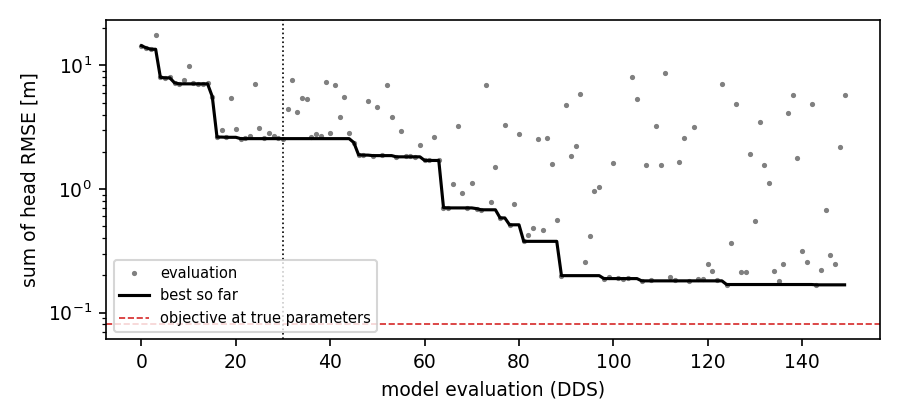
\includegraphics[width=0.8\linewidth]{figures/fig_calibration.png}
\caption{Synthetic calibration: objective against model runs.}\label{fig:calib}\end{figure}

\section{The Ostrich input file, line by line}
\begin{lstlisting}
ProgramType         DDS             # search algorithm (dynamically dimensioned search)
ObjectiveFunction   GCOP            # general constrained optimization
ModelExecutable     ./Ost-Raven.sh  # script that runs Raven in ./model
BeginFilePairs
  Liard.rvp.tpl ; model/Liard.rvp   # template -> model file with values filled in
EndFilePairs
BeginParams                         # name, start, lower, upper, transformations
  par_K_gravel   5.0  1.0  500.0  none log10 none
  par_Sy_gravel  0.10 0.05 0.35   none none  none
  par_K_till     2.0  0.01 5.0    none log10 none
EndParams
BeginResponseVars                   # values read from Diagnostics.csv
  RMSE1  model/output/Diagnostics.csv ; OST_NULL 1 4 ','  # line 1 (header = 0), column 4
  ...
EndResponseVars
BeginTiedRespVars                   # objective = sum of the RMSEs
  SUM_RMSE 4 RMSE1 RMSE2 RMSE3 RMSE4 wsum 1.0 1.0 1.0 1.0
EndTiedRespVars
BeginGCOP
  CostFunction SUM_RMSE
EndGCOP
BeginDDSAlg
  MaxIterations 150
EndDDSAlg
\end{lstlisting}
Ostrich counts the lines of \cmd{Diagnostics.csv} from 0 (the header is line 0) and its columns from 1. With
\cmd{:EvaluationMetrics NASH\_SUTCLIFFE RMSE KLING\_GUPTA} the columns are the series, the file, NSE, RMSE (column 4) and
KGE, and the four \cmd{GW\_HEAD} series are lines 1--4 when they are the model's only observations (with four monitoring
wells added to the Liard example, whose 29 streamflow series come first, lines 30--33). Check the line and column of each response in your own
\cmd{Diagnostics.csv}; they depend on the order of observations and on \cmd{:EvaluationMetrics}. To combine heads and streamflow, add NSE or KGE responses of the hydrographs with suitable weights.

\section{Troubleshooting}\label{ch:trouble}
\begin{table}[!htbp]\centering
\caption{Messages and symptoms, with their causes and remedies.}
\begin{tabular}{P{0.36\linewidth}P{0.588\linewidth}}\toprule\hdr
Message or symptom & Cause and remedy\\\midrule
``cannot load MODFLOW 6 library'' & run \cmd{python tools/get\_mf6.py} of RavenHydroFramework-extra, or set \cmd{:MF6Library} or \cmd{RAVEN\_MF6\_LIB} to the full path of \cmd{libmf6}; the message lists the places searched\\
``MODFLOW 6 stopped the run during \dots'' & MODFLOW found an input error inside its library; the message (also in \cmd{Raven\_errors.txt}) quotes the error report of \cmd{<output>/mf6/mfsim.lst}\\
``GeoJSON file \dots\ is in EPSG:\emph{n}'' / ``\dots\ outside the longitude/latitude range'' & a projected input file: give \cmd{:InputCRS} (Section~\ref{sec:inputcrs})\\
``layer \dots\ starts dry'' (warning) & the initial heads leave a whole layer dry; start from \cmd{:GWInitialization STEADY\_STATE}, a smaller \cmd{INITIAL\_HEAD\_DEPTH} or \cmd{:InitialGWHeads}\\
``HRU \dots\ has an AQUIFER\_PROFILE but no polygon'' & HRU IDs in the GeoJSON do not match the \cmd{.rvh}; check the ID field name\\
``does not overlap any active groundwater cell'' & the HRU is too small for the grid or sits where bedrock is at the surface; reduce \cmd{:GridCellSize} or \cmd{:MinCellCoverage}, or check the bedrock map\\
``polygon area \dots\ differs from .rvh AREA'' & information only; volumes are always consistent\\
``process \dots\ removes water from GROUNDWATER'' & a Raven process drains \cmd{GROUNDWATER} in a coupled HRU; restrict it with \cmd{:-->Conditional}\\
``process \dots\ sends water to GROUNDWATER in HRU \dots\ which has no AQUIFER\_PROFILE'' & that water would leave the model; restrict the process\\
``MODFLOW 6 did not converge'' & start from a steady state or realistic heads; raise \cmd{:SolverMax\allowbreak OuterIterations}; increase \cmd{SEEPAGE\_SMOOTHING\_DEPTH}; check for extreme parameter contrasts\\
Well rate is zero (``no :WellFlowRate time series'') & the \cmd{:WellFlowRate} block is missing, or its ID does not match an ID in \cmd{:Wells}\\
``reservoir \dots\ has no :SeepageParameters'' / ``no coupled lake HRU'' & add \cmd{:SeepageParameters}; give the lake HRU an \cmd{AQUIFER\_PROFILE}\\
``running more time steps than the MODFLOW 6 simulation holds'' & \cmd{:Duration} or \cmd{:TimeStep} is inconsistent; rerun\\
Water table far above the land surface & \cmd{SEEPAGE\_LEAKANCE} too small, or $K$ too low for the recharge\\
Aquifer steadily emptying for years & initial heads too high; use a steady-state start or a longer spin-up\\\bottomrule
\end{tabular}
\end{table}

\section{Frequently asked questions}
\paragraph{Do I need MODFLOW experience?} No. Raven writes and runs the MODFLOW model. It helps to know the concepts of
Chapter~\ref{ch:c2}; the generated files can be inspected by anyone who knows MODFLOW.
\paragraph{Can only part of my watershed have groundwater?} Yes. Only HRUs with an \cmd{AQUIFER\_PROFILE} are coupled; all
others run exactly as they do without groundwater.
\paragraph{Can two aquifer systems exchange water?} Yes, when their cells touch: lateral flow between neighbouring profiles and
leakage between layers are computed by MODFLOW like any other flow.
\paragraph{What happens where the water table reaches the surface?} The seepage drains return the water to Raven, where it
follows Raven's processes (for example baseflow to the river).
\paragraph{Can the aquifer take more water than a river carries?} Not from a river Raven builds: the supply limit caps
each river cell's largest possible loss at its share of the reach's flow at the start of the step, and the loss is taken
from the reach's runoff, inflow and outflow, so the outflow leaving the watershed falls by it. Only a reach whose flow stops within the step
can leave part of its loss to be carried to the next step (warned about; the loss carried at the end of the run is a run
total of \cmd{GWModelSummary.txt}). An existing model's stream package keeps its own
conductance and has no supply limit (Section~\ref{sec:extlimits}): a losing reach can take more than the channel holds, and
the part the channel cannot supply is carried to the next step (\emph{river loss carried to next step}; exactly accounted).
Example~B does this for months: the carry reaches about $10^{8}$~m$^3$ and is repaid by the end of the run.
\paragraph{How do I restart a long run?} Use \cmd{solution.rvc} of the finished run as the \cmd{.rvc} of the next, with
\cmd{:StartDate} set to the end of the first run. A coupled run continued this way carries on exactly
(Section~\ref{sec:hotstart}); a run without groundwater continues from Raven's 5-decimal states.
\paragraph{How fine should the grid be?} Fine enough that valleys and well spacings span two or three cells
(Section~\ref{ch:grid}). Coarser grids run faster.
\paragraph{Does frozen ground limit recharge?} Recharge is whatever Raven's processes send to \cmd{GROUNDWATER}, so frozen
ground acts on it through Raven's own process choices (a \cmd{:FrozenGround} process, infiltration and percolation methods
that respond to frozen soil); the coupling adds no frozen-ground control of its own.
\paragraph{How long a spin-up do I need?} Start from a steady state with the long-term mean recharge, then check that
\emph{storage release} in \cmd{GWBudget.csv} averages near zero over the first years; large, slow aquifers may need decades.
\paragraph{Can I see the head everywhere, not only at wells?} Yes: \cmd{mf6/gwf.hds} (MODFLOW binary, readable with FloPy)
every \cmd{:HeadSaveFrequency} steps, or \cmd{GWHeads.nc} with \cmd{:WriteNetCDFHeads}.
\paragraph{Does the coupling change results for my other subbasins?} Only through the rivers: groundwater discharge or losses
in coupled subbasins change the flow passed downstream.
\paragraph{Can I use it in an ensemble or with Ostrich?} Yes; each ensemble member rebuilds and restarts MODFLOW, and aquifer
parameters are ordinary \cmd{.rvp} values.
\paragraph{What if MODFLOW stops the program?} Read \cmd{<output>/mf6/mfsim.lst}; it names the file and value MODFLOW rejected.
